\chapter{Software design}

\label{ch:Software design}

\setlength{\parindent}{4em}
\setlength{\parskip}{1em}
\renewcommand{\baselinestretch}{1.5}

\section{System architecture}

\hspace{1.5cm}In our project, we use two algorithms to stimulate the subject. First, we use ERPs which is different in stimulating time. Second is SSVEP which difference in stimulating frequency. This is our system architecture design.

\begin{figure}[ht]
	\centering
	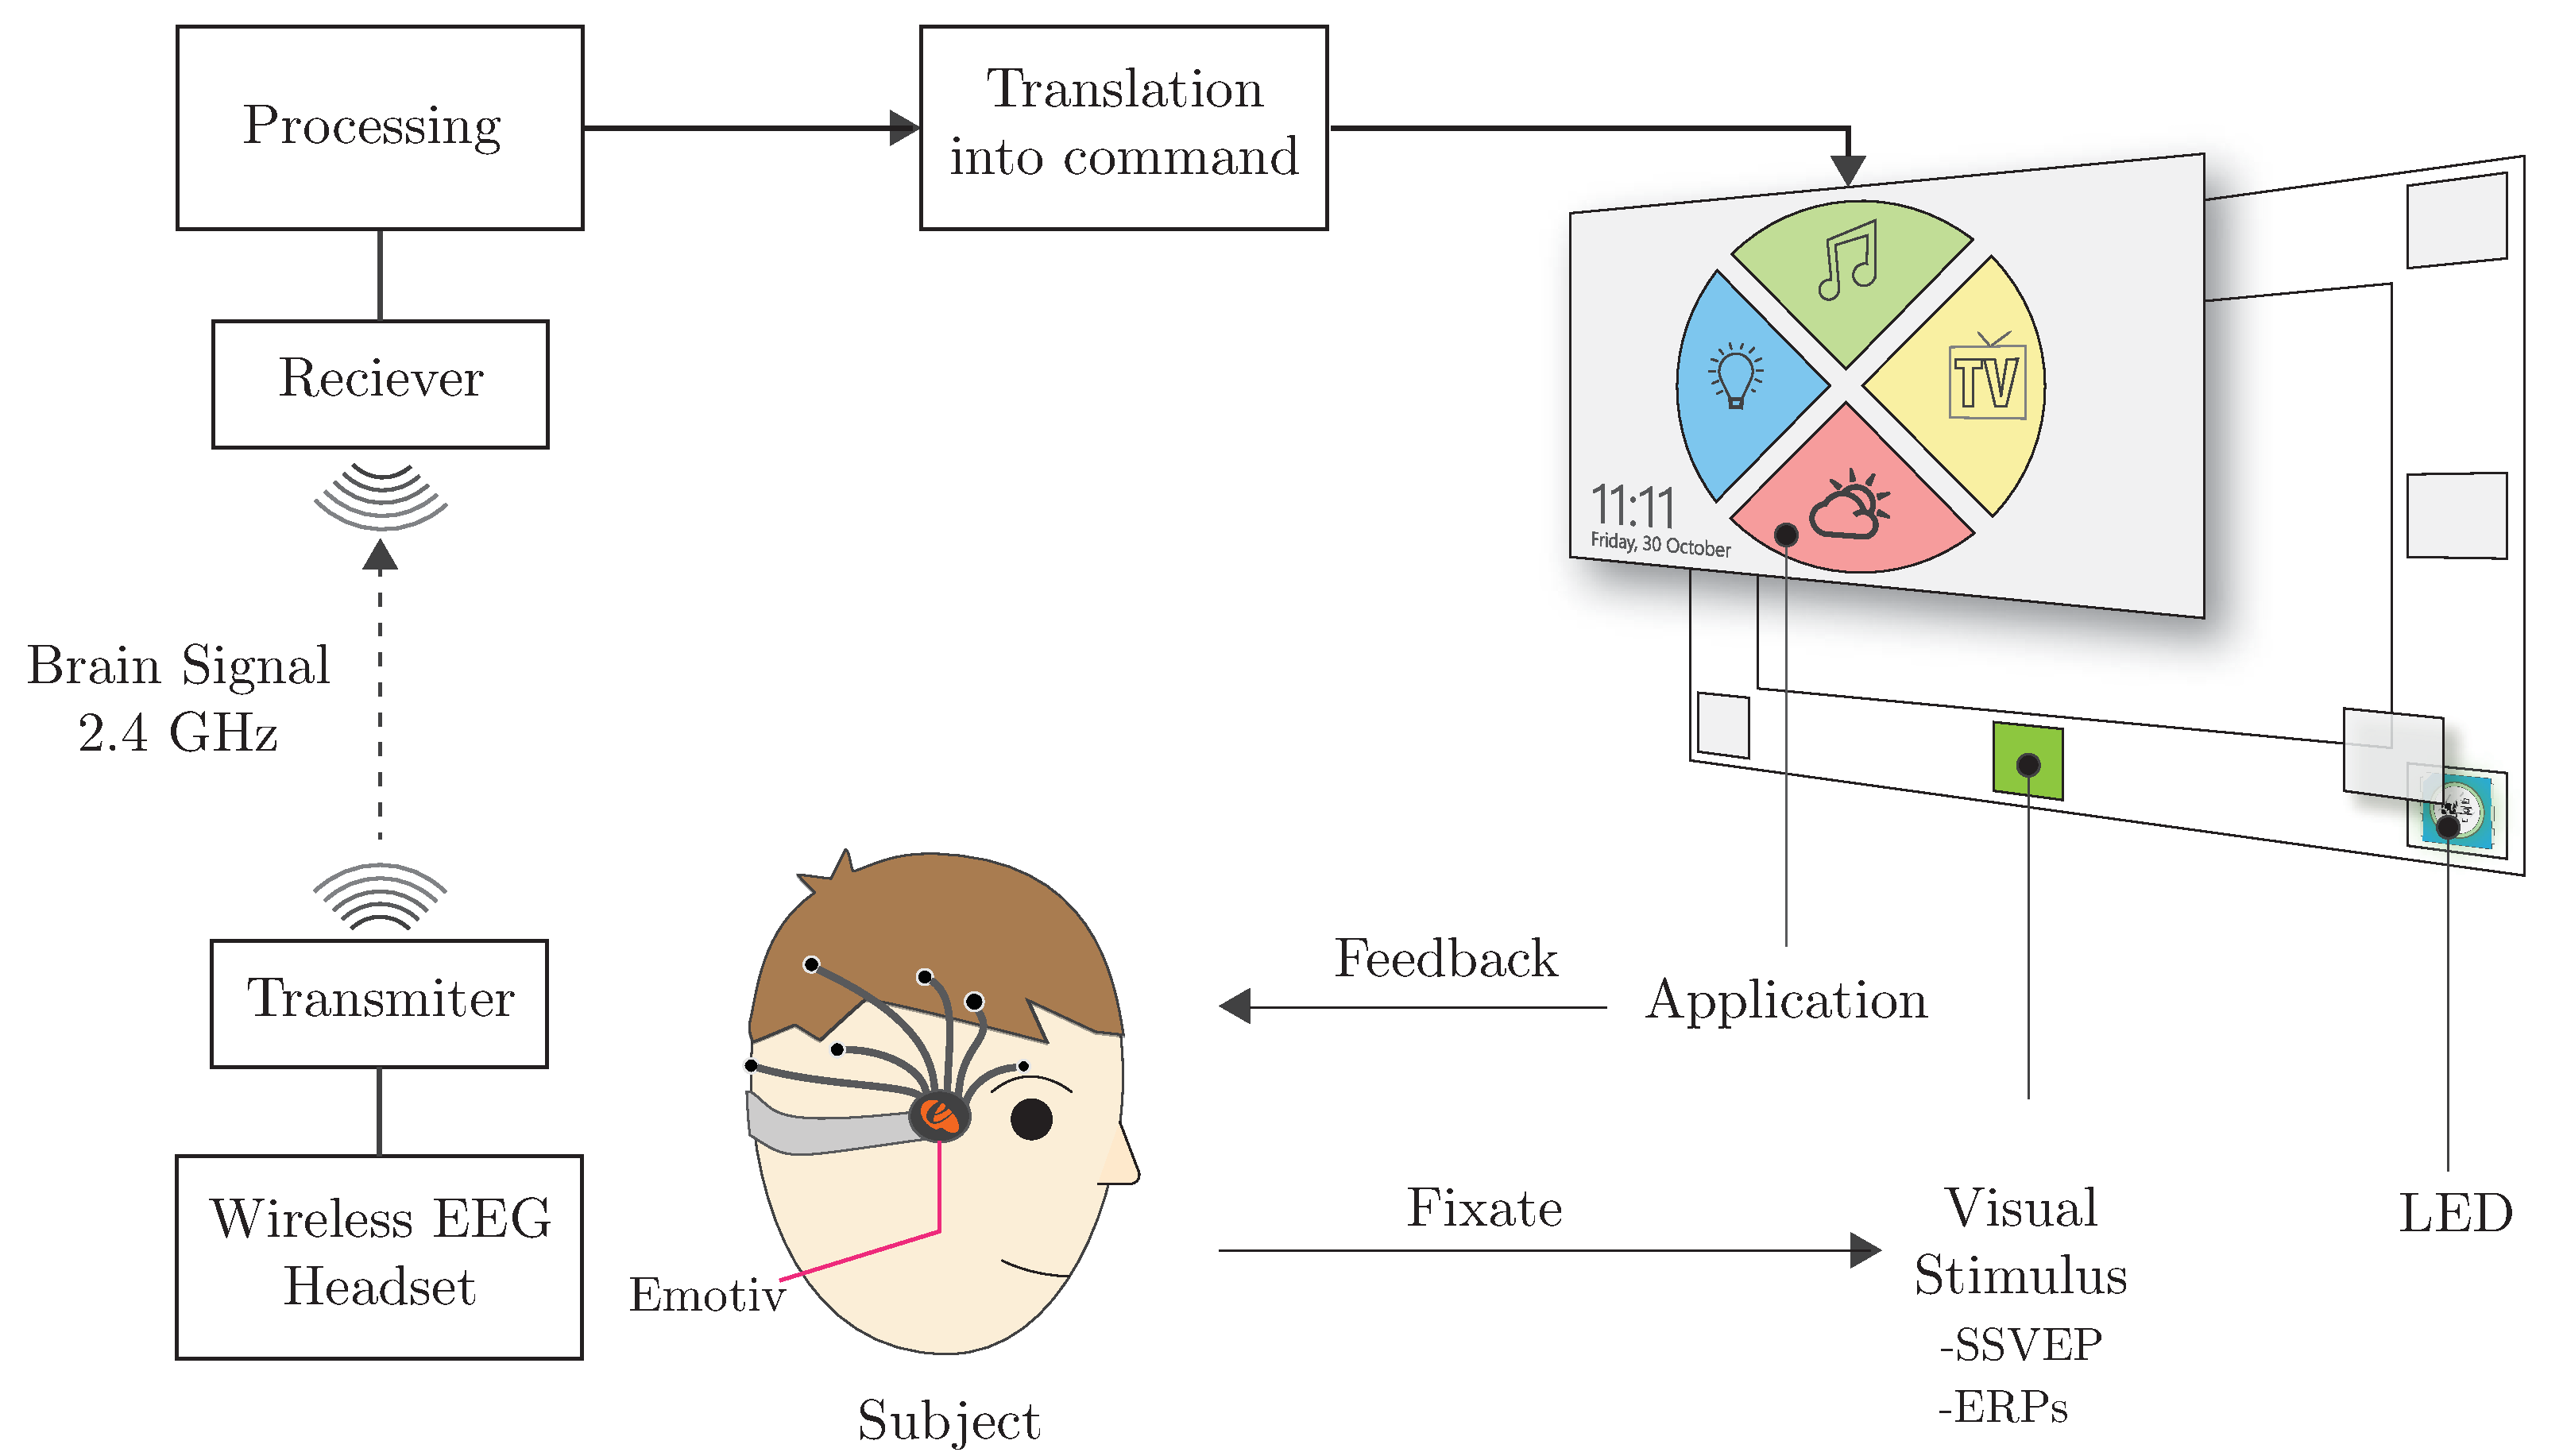
\includegraphics[scale = 0.28]{chapter5/architec.pdf}
	\caption{System architecture design}
\end{figure}

\begin{figure}[ht]
	\centering
	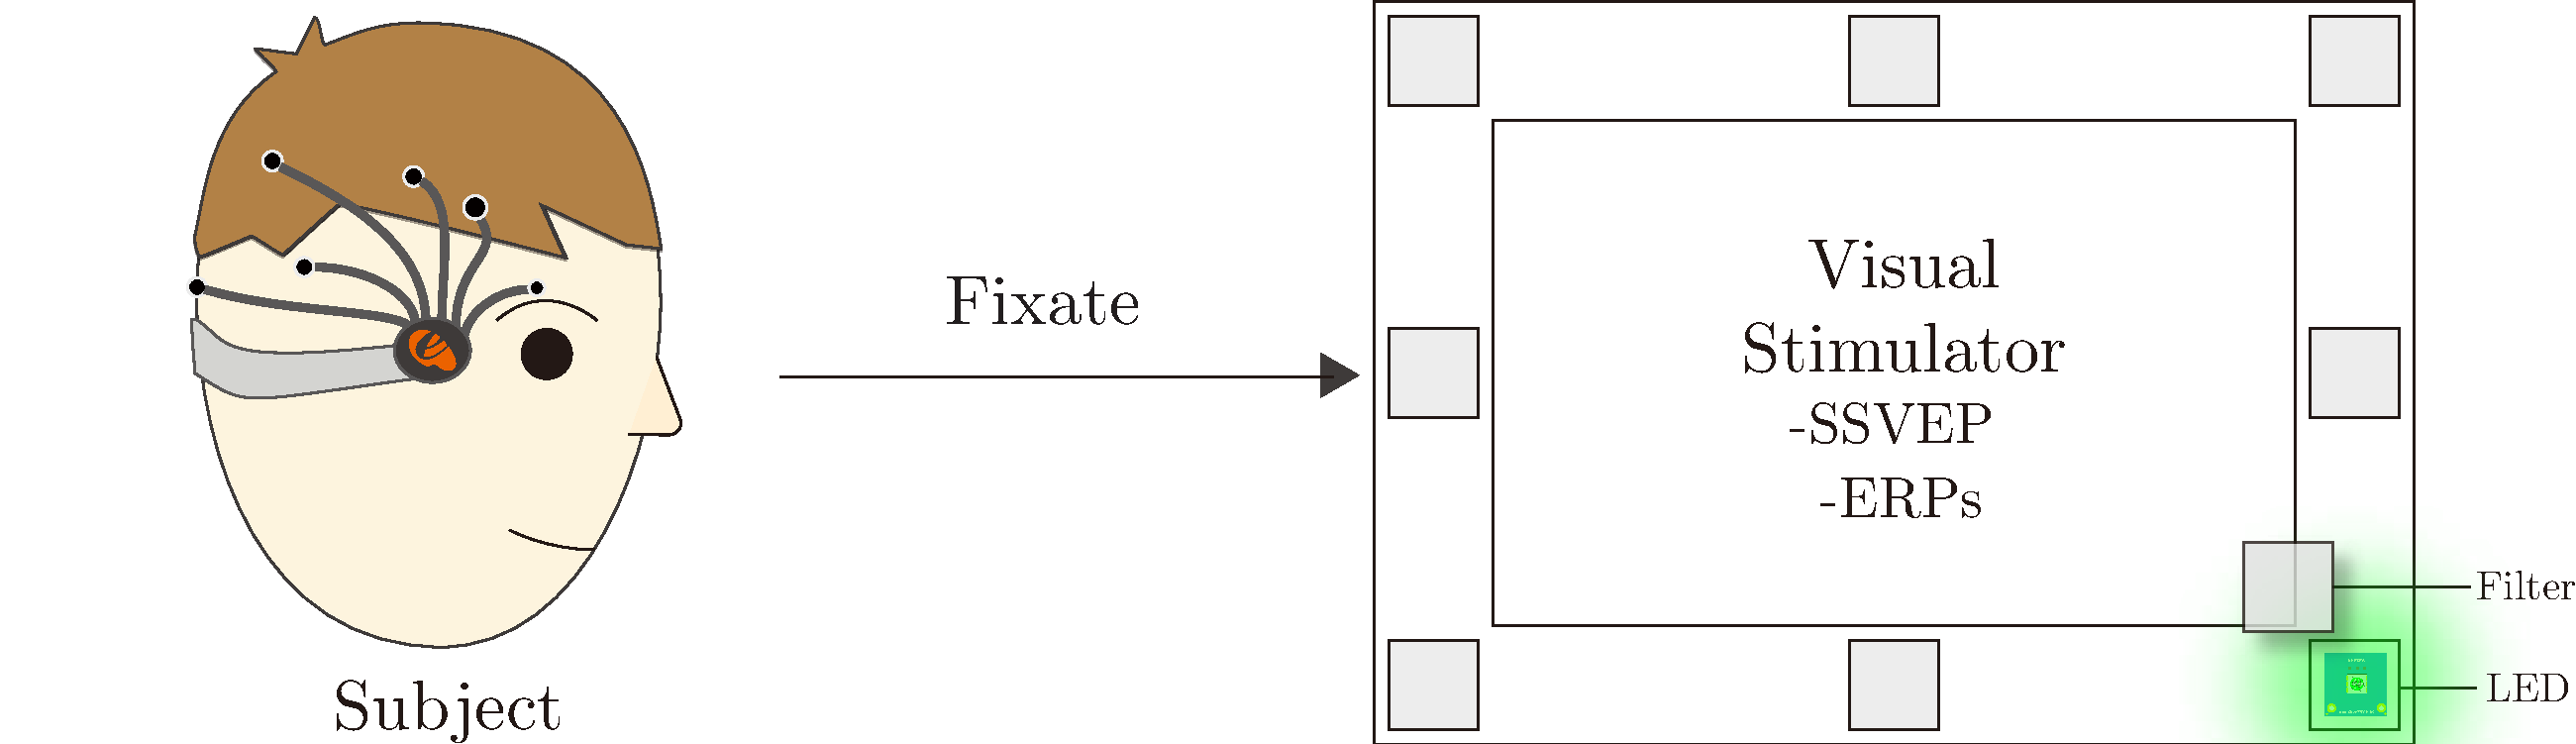
\includegraphics[scale = 0.5]{chapter5/frame_led.pdf}
	\caption{System architecture design}
\end{figure}

\subsection{Visual stimulator}

\hspace{1.5cm}In each visual stimulator, a target is contained with one LED to make light stimuli. We use Gravitech Gerora RGB LEDs to be a light source, which is controlled by Arduino Uno.  The parameter of LEDs is consisted of flickering frequency, duty cycles, intensity, color, status tell it is turned on or off. It can use in ERPs and SSVEP method. 

In ERPs method, we use visual stimulator with four targets, because it takes a lot of time to surely classify. To make a classification process fast, The optimal number of target for the program to operate is four.

In SSVEP method, we use visual stimulator with eight targets. Because it takes less time than ERPs. The functional is similar to ERPs method, but it adds four function shortcuts.

\subsection{Wireless EEG Headset}
\hspace{1.5cm}To use the application subject has to fixate at the stimuli target which has different functional. Before the experiment, the subject has to equip the EEG recording headset. Then subject has to fixate at the stimulation, the brain will generate a ERPs or SSVEP, the wireless headset will record it. and we can use for classification. Then the recorded brainwave will be transmitted via 2.4GHz wireless for further processing.

\subsection{Processing}
\hspace{1.5cm}The processing process is receiving a recorded EEG signal result from the wireless headset via the 2.4GHz wireless receiver. The ERPs and SSVEPs will use a different algorithm to process. To know which target subject fixate at, in ERPs, we will use P300 theory. In SSVEP, we will use Fourier Transform. Then it will send classification result to translate into command.
\subsection{Translate into command}
After we know which target subject fixate at, it will be translate into command. Because each target is associated with one function, then it will match the target from processing with the function. And it will tell the application to do that function. the subject will get feedback that it do function that they want.

\newpage
\section{Class Diagram}
\
\begin{figure}[ht]
	\centering
	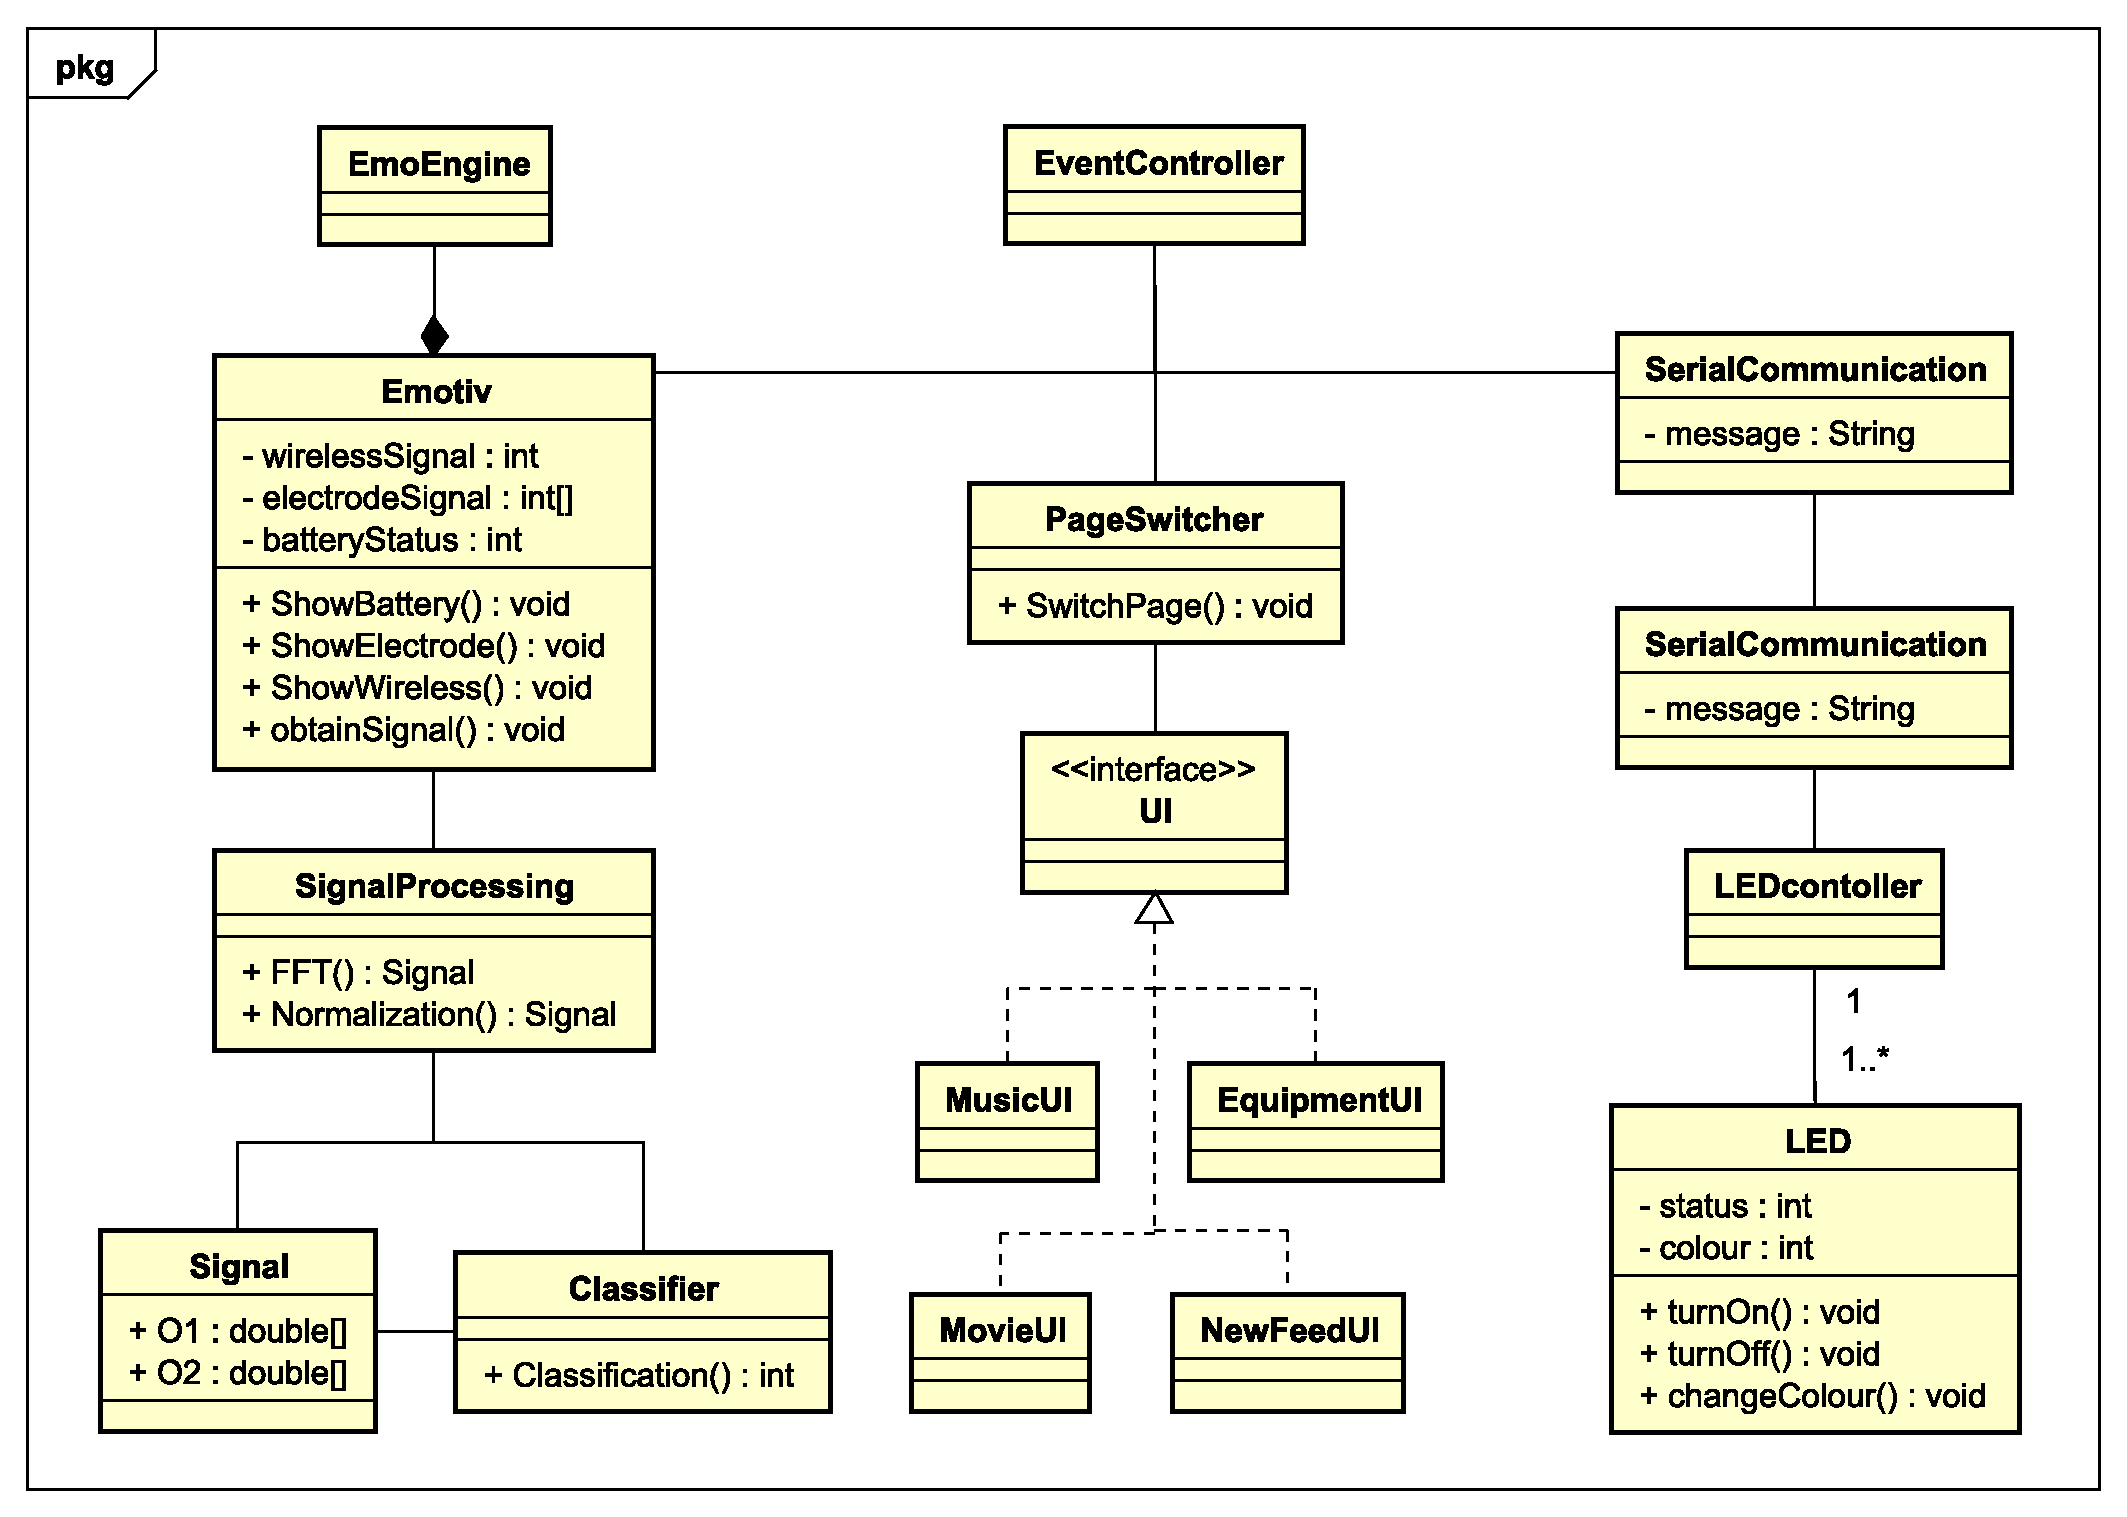
\includegraphics[width=\textwidth]{chapter5/Class.pdf}
	\caption{Visual Stimulator}
\end{figure}

Class diagram description, starting with the most importance class, EventController, it is connecting Emotiv headset to system, PageSwitcher, and Serial communication classes together to make a program work in unison,

EmoEngin is a library use for connecting our program to an Emotiv headset. Emotiv class is a substitute of a headset. It has a property of wireless signal quality, electrode contact quality, battery level which is obtained via EmoEngin. The signal class represents the EEG signal that obtains from Emotiv headset. In this project is use the only occipital channel, so the attribute is only O1 and O2. The SignalProcessing class contains an algorithm to process EEG signal to a frequency domain to perform analysis and to have standardized by normalization. The Classifier class is to classify a feature from the processed signal. the result will tell which flicker user fixate at. then it will send the result to EventController to do further step.

After obtaining the result from classification, the EventController will tell the page switcher to change page. EquipmentUI, MusicUI, MovieUI, NewfeedUI, all the user interface pages inherit from UI interface for PageSwitcher can easily control, also easily add new UI page.

The SerialCommunication Class is a class that connects to Arduino via Serial port. It will encode a control command to Arduino to control the LEDs , which Arduino part also have a SerialCommunication class to decode the command that receives via a serial port. Then it will send the command to LEDController to control the LEDs via Arduino's pin. LED class represents for an LEDs. It can control to turn on or off , change color, and frequency.